\section{Лекция 18}
\begin{theorem}
    Пусть $\overline{\Delta}\subset \Omega$ --- треугольник, $(P,Q)$ --- дифференцируемое векторное поле в $\Omega,\ Q'_x-P'_y\in \mathcal{C}(\Omega)$. Тогда
    \[\oint\limits_{\gamma}P\ dx+Q\ dy=\iint\limits_{\overline{\Delta}}(Q'_x-P'_y) dxdy\]
\end{theorem}
\begin{proof}
    Пусть
    \[M=\oint\limits_{\gamma}P\ dx-+Q\ dy-\iint\limits_{\overline{\Delta}}(Q'_x-P'_y)\ dxdy\]
    Разбили наш треугольник на 4 треугольника. $\exists\ \Delta_1$:
    \[\oint\limits_{\gamma_1}P\ dx+Q\ dy-\iint\limits_{\overline{\Delta_1}}(Q'_x-P'_y)\ dxdy\geq \frac{M}{4}\]
    Получили последовательность вложенных треугольников
    \[\Delta_0\supset\Delta_1\supset\Delta_2\subset\dots\]
    где диаметр $D_n=\frac{D}{2^n},\ P_n=\frac{P}{2^n},\ S_n=\frac{S}{4^n}$
    \[P(x,y)=P(x_0,y_0)+P'_x(x_0,y_0)\cdot (x-x_0)+P'_y(x_0,y_0)\cdot (y-y_0)+\alpha_1(x,y)\cdot \sqrt{(x-x_0)^2+(y-y_0)^2}\]
    \[\int\limits_{\gamma_n}P\ dx+Q\ dy-\int\limits_{\overline{\Delta}_n}(Q'_x-P'_y)\ dxdy\geq\frac{M}{4^n}\]
\begin{lemma}
    \begin{enumerate}
        \item \[\oint\limits_{\gamma}x\ dx=\oint\limits_{\gamma}y\ dy=0\]
        \item \[\oint\limits_{\gamma}y\ dx=\oint\limits_{\gamma}x\ dy=S(\Delta ABC)\]
    \end{enumerate}
\end{lemma}
\begin{proof}
    \begin{enumerate}
        \item Предъявим потенциал $U=\frac{x^2}{2} \Rightarrow U'_x=x,\ U'_y=0$ аналогично для второго интеграла.
        \item Покажем, что
        \[-\oint\limits_{\gamma}y\ dx=S(\Delta ABC)\]
        там мы рисуем треугольник и показываем что интеграл не изменяется при параллельном переносе. Для движения по горизонтали очевидно там что то из интеграла Стильтьеса, а по вертикали смотрим на интегральную сумму
        \[\sigma=\sum\limits_{i=1}^{n}(y_{\text{нижн}_i}-y_{\text{верх}_i})\Delta x_i\]
        поэтому при сдвиге ничего не меняется.
        тут много картинок(((
    \end{enumerate}
\end{proof}
\begin{multline*}
    \int\limits_{\gamma_n}P\ dx+Q\ dy=\int\limits_{\gamma_n}(P'_y(x_0,y_0)\cdot(y-y_0)+\alpha_1(x,y)\cdot \sqrt{(x-x_0)^2+(y-y_0)^2})dx+\\
    +(Q'_x(x_0,y_0)\cdot (x-x_0)+\alpha_2(x,y)\cdot \sqrt{(x-x_0)^2+(y-y_0)^2}\ dy)=\\
    =(Q'_x(x_0,y_0)-P'_y(x_0,y_0))\cdot S_n+\int\limits_{\gamma_n}\sqrt{(x-x_0)^2+(y-y_0)^2}\cdot (\alpha(x,y)dx+\alpha_2(x,y)dy)
\end{multline*}
\[\left|\int\limits_{\gamma} f_1\ dx+ f_2\ dy\right|\leq \max\limits_{\gamma}\sqrt{f_1^2+f_2^2}\cdot |\gamma|\]
\[|\dots|\leq \max\limits_{\gamma_n} \sqrt{(x-x_0)^2+(y-y_0)^2}\cdot \sqrt{\alpha_1^2+\alpha_2^2}-|\gamma_n|\leq \overline{\overline{o}}(1)D_n\cdot P_n=\overline{\overline{1}}\cdot \frac{P\cdot D}{4^n}\]
$\forall \epsilon>0\ \exists\ \delta>0,\ \sqrt{(x-x_0)^2+(y-y_0)^2}<\delta$:
\[|(Q'_x-P'_y)(x,y)-(Q'_x-P'_y)(x_0,y_0)|<\epsilon\]
\begin{multline*}
    \left|\iint\limits_{\Delta_n}(Q'_x-P'_y)\ dxdy-\iint\limits_{\Delta_n}(Q'_x-P'_y)(x_0,y_0)\ dxdy\right|=\\
    =|\iint\limits_{\Delta}(Q'_x-P'_y)(x_0,y_0)-(Q'_x-P'_y)(x_0,y_0)\ dxdy|\leq \epsilon\cdot S_n
\end{multline*}
Итак
\[\left|\int\limits_{\gamma_n}P\ dx+Q\ dy-\iint\limits_{\Delta_n}(Q'_x-P'_y)\ dxdy\right|\leq \overline{\overline{o}}(1)\cdot D_n\cdot P_n+\overline{\overline{o}}(1)\cdot S_n=\overline{\overline{o}}\left(\frac{1}{4^n}\right)\]
\end{proof}
тут про индекс кривой.\\
Теперь общий случай (доказывать его конечно же не будем)
\begin{theorem}
    Пусть $\gamma$ --- спрямляемая кривая. Тогда
    \[\int\limits_{\gamma}P\ dx+Q\ dy=\iint\limits_{\R^2}(Q'_x-P'_y)\cdot \text{ind}_{\gamma}\ dxdy\]
\end{theorem}
Мы же докажем для замкнутой ломаной без пересечений.
\begin{theorem}
    Пусть $\Lambda$ --- замкнутая ломаная без самопересечений в $\Omega,\ P,Q\in \mathcal{D}(\Omega),\ Q_x'-P_y'\in \mathcal{C}(\Omega)$. тогда
    \[\oint\limits_{\Lambda}P\ dx+Q\ dy=\iint\limits_{\Phi}(Q'_x-P'_y)\ dxdy\]
\end{theorem}
\begin{proof}
    Хотим свести задачу к предыдущей и разбить многоугольник на треугольники:
    \begin{enumerate}
        \item Если многоугольник выпуклый, то преведем диагонали из одной вершины и получим что нужно
        \item Если многоугольник не выпуклый то проводим семейство параллельных прямых (достаточно частно) и разрезаем этот многоугольник на выпуклые многоугольники.
    \end{enumerate}
\end{proof}
\begin{consequense}
    Пусть $\gamma$ --- такая замкнутая простая кривая, что для нее существует последовательность вписанных простых ломаных с максимальной длиной отрезков стремащихся к нулю.
\end{consequense}
Теперь рассказываем ради чего это все
\begin{multline*}
    \int\limits_{\gamma}f(z)\ dz=\int\limits_{\gamma} u(x,y)+i\cdot v(x,y)\ d(x+iy)=\\
    =\left(\int\limits_{\gamma}u(x,y)\ dx-v(x,y)\ dy\right)+i\cdot \left(\int\limits_{\gamma}v(x,y)\ dx+u(x,y)\ dy\right)
\end{multline*}
\begin{definition}
    
\end{definition}
\begin{theorem}
    Пусть $f\in \mathcal{A}(\Omega), \gamma$ --- замкнутая спрямляемая ограниченная кривая. На множестве $\Phi\subset \Omega$ справедлива формула Грина. Тогда
    \[\oint\limits_{\gamma}f(z)\ dz=0\] 
\end{theorem}
\begin{proof}
    \[\zeta=\lim\limits_{z\to z_0}\frac{f(z)-f(z_0)}{z-z_0} \Leftrightarrow f(z)-f(z_0)=\zeta\cdot (z-z_0)+\overline{\overline{o}}(1)\cdot (z-z_0)\]
    \[\begin{cases}
        u(x,y)-u(x_0,y_0)=\xi(x-x_0)-\eta(y-y_0)+\overline{\overline{o}}(1)\cdot \sqrt{(x-x_0)^2+(y-y_0)^2},\\
        v(x,y)-v(x_0,y_0)=\eta(x-x_0)-\xi(y-y_0)+\overline{\overline{o}}(1)\cdot \sqrt{(x-x_0)^2+(y-y_0)^2}
    \end{cases}\]
    \begin{multline*}
        (\xi+i\eta)((x-x_0)+i(y-y_0))=\\
        =\xi(x-x_0)-\eta(y-y_0)+i(\eta(x-x_0)+\xi(y-y_0))
    \end{multline*}
\end{proof}
\begin{example} [Сапог Шварца] $\\$
    Рассмотрим цилиндр
    $S_{\text{бок}}=2\pi R\cdot H$ разрежем его на $m$ слоев
    Впишем в верхнюю окружность правильный пятиугольник потом спускаемся на слой ниже и рисуем пятиугольнимк в противофазе
    прикол тут будет в том что при одном стремлении m n к бесконечности мы получим площадь поверхности а при другом нет
    в следующий раз проверим это
\end{example}
\begin{center}
    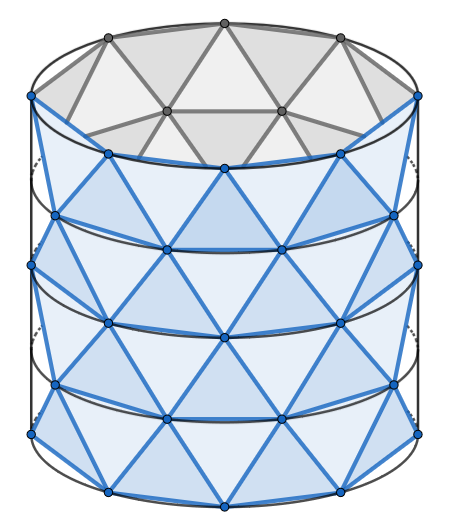
\includegraphics[width=0.4\textwidth]{Images/Sapog.png}
\end{center}
\newpage